\section{Soluțiile problemelor}
\textbf{Domain file}\newline\newline

\inputminted[linenos]{python}{code/all-out.pddl}

\newline
În domain definim matricea de lumini și vecini:
light-on sunt luminile aprinse(cu un singur număr), au not în față dacă sunt stinse, iar neighbor este format din 2 numere deoarece conține numărul luminii căreia este vecin și numărul său.
Acțiunea este aceea de a stinge lumina: not(light-on ?x) pentru toate luminile și vecinii lor.
\newline\pagebreak
\newpage
\textbf{AllOut 4x4:}\newline\newline
\inputminted[linenos]{python}{code/all-out-p02.pddl}
\newline\newline
\newline\pagebreak
 \subsection{Case 1}
 \newline
 \newline
(not(light-on light1))  
(light-on light2)  
(not(light-on light3))  
(not(light-on light4))
\newline
(light-on light5)  
(light-on light6)  
(light-on light7)  
(not(light-on light8))
\newline
(not(light-on light9)) 
(light-on light10) 
(not(light-on light11)) 
(not(light-on light12))
\newline
(not(light-on light13)) 
(not(light-on light14)) 
(not(light-on light15)) 
(not(light-on light16))
\newline
\newline
\begin{figure}[h]
\centering

\includegraphics[width=6cm]{text/images/pic3.jpeg}\\
\newline
\caption{AllOut 4x4}
\end{figure} \newline \newline

\newline\newline
\newline
 \subsection{Case 2}
 \newline
 \newline
((light-on light1)  
(not(light-on light2))  
(not(light-on light3))  
(not(light-on light4))
\newline
(not(light-on light5))  
(light-on light6)  
(light-on light7)  
(not(light-on light8))
\newline
(not(light-on light9))  
(light-on light10) 
(not(light-on light11)) 
(not(light-on light12))
\newline
(not(light-on light13)) 
(not(light-on light14)) 
(not(light-on light15)) 
(not(light-on light16))
\newline
\begin{figure}[h]
\centering

\includegraphics[width=6cm]{text/images/pic2.jpeg}\\
\newline
\caption{AllOut 4x4}
\end{figure} \newline \newline

\pagebreak

\textbf{AllOut 5x5:}\newline\newline
\inputminted[linenos]{python}{code/all-out-p01.pddl}
\pagebreak

\subsection{Case 1}
 \newline
 \newline
(not(light-on light1)) 
(not(light-on light2)) 
(not(light-on light3)) 
(not(light-on light4)) 
(not(light-on light5))
\newline
(not(light-on light6)) 
(not(light-on light7)) 
(not(light-on light8)) 
(not(light-on light9)) 
(not(light-on light10))
\newline
(not(light-on light11)) 
(not(light-on light12)) 
(not(light-on light13)) 
(not(light-on light14)) 
(not(light-on light15))
\newline
(not(light-on light16)) 
(not(light-on light17)) 
(light-on light18) 
(light-on light19) 
(light-on light20)
\newline
(not(light-on light21)) 
(light-on light22) 
(not(light-on light23)) 
(light-on light24) 
(not(light-on light25))
\newline
\newline
\begin{figure}[h]
\centering
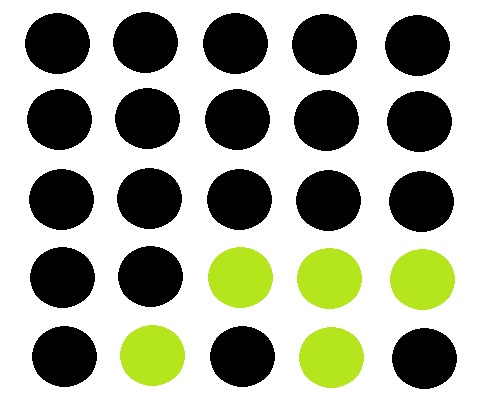
\includegraphics[width=6cm]{text/images/pic5.jpeg}\\
\newline
\caption{AllOut 5x5}
\end{figure} \newline \newline

\newline\newline
\newline
 \subsection{Case 2}  \newline
 \newline
 \newline
  \newline
(not(light-on light1)) 
(light-on light2) 
(not(light-on light3)) 
(not(light-on light4)) 
(not(light-on light5))
 \newline
(light-on light6) 
(light-on light7) 
(light-on light8) 
(not(light-on light9)) 
(not(light-on light10))
 \newline
(not(light-on light11)) 
(light-on light12) 
(not(light-on light13)) 
(light-on light14) 
(not(light-on light15))
 \newline
(not(light-on light16)) 
(not(light-on light17)) 
(light-on light18) 
(light-on light19) 
(light-on light20)
 \newline
(not(light-on light21)) 
(not(light-on light22)) 
(not(light-on light23)) 
(light-on light24) 
(not(light-on light25))
\newline
\begin{figure}[h]
\centering

\includegraphics[width=6cm]{text/images/pic4.jpeg}\\
\newline
\caption{AllOut 5x5}
\end{figure} \newline \newline

\pagebreak